\documentclass[a4paper,12pt]{article}
\usepackage[latin1]{inputenc}
\usepackage[spanish]{babel}
\usepackage{amsmath}
\usepackage{graphicx}
\setlength{\textheight}{250mm}
\setlength{\textwidth}{165mm}
\setlength{\topmargin}{-15mm}
\setlength{\oddsidemargin}{0pt}
\pagestyle{empty}

\begin{document}

\def\bm#1{{\mbox{\boldmath $#1$}}}
\def\eqdef{\buildrel \rm def \over =}
\def\signo{\mathop{\rm signo}\nolimits}

\mbox{}\vspace*{-20mm}

{\centering
{\small\sc Escuela T�cnica Superior de Ingenieros de Caminos, Canales y Puertos (Madrid)}\\*[4mm]
{\Large\bf M�todo de los Elementos Finitos (Curso 20-21)}\\*[4mm]
EXAMEN FINAL ORDINARIO (8 de febrero de 2021)
}

% \vspace{4mm}

% ENUNCIADO
Se considera el modelo de elementos finitos de una viga cuyos extremos
est�n comprendidos entre $x=0$ y 
$x=18$ m, siendo su secci�n transversal la que se indica en la figura.
En el extremo $x=18$ hay una carga puntual aplicada, seg�n se indica en la
figura, de valor $F=500$ kN. Tambi�n act�a el peso propio que es el
correspondiente a un hormig�n de densidad $\rho=2500$ kg/m$^3$ (se tomar� $g=10$ m/s$^2$).
Las propiedades mec�nica son: $E=32$ GPa y $\nu=0.2$.

Todos los nodos situados en el plano $x=0$ tienen los
movimientos impedidos.

La discretizaci�n de la secci�n transversal es la que se muestra en la figura,
siendo todos los elementos del modelo hexaedros de $8$ nodos. En direcci�n
longitudinal (seg�n $Ox$) hay 68 elementos.
Se utilizar�n elementos hexa�dricos con formulaci�n de deformaciones mejoradas
supuestas (``enhanced assumed strain'').

Se pide:
\begin{enumerate}
	\item Hacer el modelo de elementos finitos correspondiente, y contestar a las
	preguntas del cuestionario disponible en el sitio Moodle de la asignatura.
	\item Cargar en el enlace correspondiente de Moodle el fichero {\tt FeapAAAA.eps}
	con los contornos de movimientos en direcci�n $z$
\end{enumerate}
{\bf NOTA:}
\begin{enumerate}
	\item El bloque $1$ (rojo) est� discretizado con $68$ elementos en direcci�n $x$, $27$ elementos en direcci�n
	$y$ y $3$ elementos en direcci�n $z$. El bloque $2$ (azul) est� discretizado con $68$ elementos en direcci�n $x$, $3$ elementos en direcci�n $y$ y $12$ elementos en direcci�n $z$. Todos los elementos son
	cuadril�teros bilineales.
\end{enumerate}


\vspace{5mm}
\begin{center}
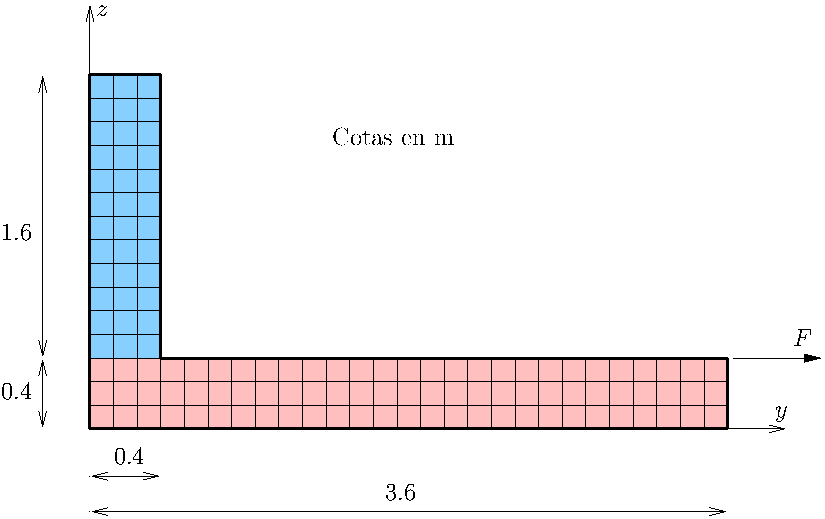
\includegraphics[width=0.4\textheight]{ejerci2}
\vspace{1cm}

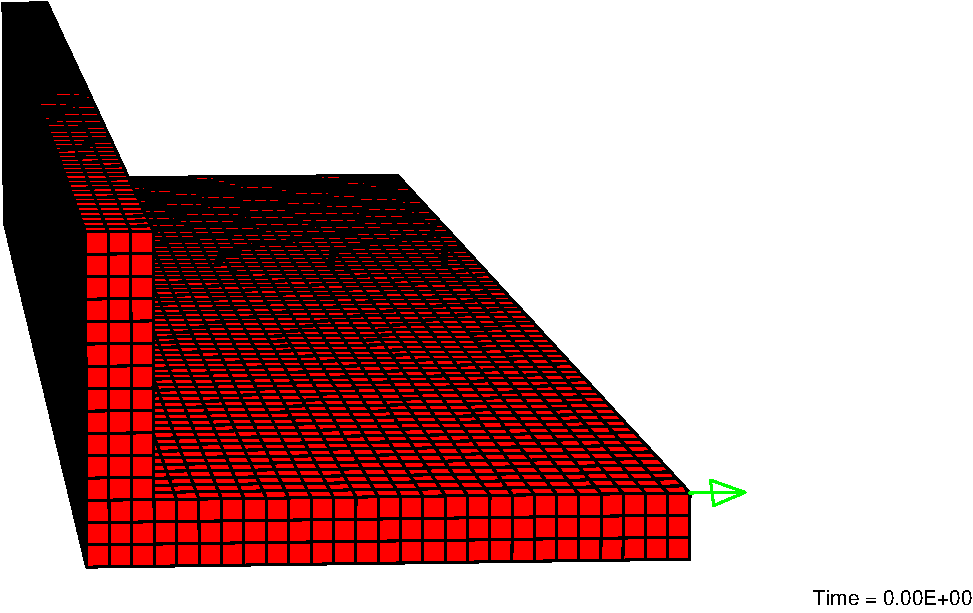
\includegraphics[width=0.45\textheight]{malla-F}
\end{center}

\end{document}
